\section{第IIIポジションと調弦}
\begin{center}
\begin{tabular}{|lcl|}
\hline
この章の基礎練習 & : & 1. 開放弦の練習 2. 「\ref{half_scale}」「\ref{1st_scale}」「\ref{2nd_scale}」「\ref{4th_scale}」の音階練習 3. 「マイスタージンガー」\\
この章の修了課題 & : & 1. 「\ref{3rd_scale}」の音階練習を正しい音程で暗譜して演奏できる\\
               &   & 2. 独力でコントラバスを調弦できる\\
               &   & 3. 「ます」を正しい音程で暗譜して演奏できる\\
\hline
\end{tabular}
\end{center}

\begin{flushleft}
\begin{minipage}{300pt}
\subsection{第IIIポジションの位置}
\ \ \ \ 前の章では第IVポジションを勉強しました。この章で扱う位置がわ
からなくなったら、「第IVの1 \(=\) 第IIIの4」という
関係を使って位置を確認しましょう。

\subsection{第IIIポジションで取れる音}
\begin{music}
\nostartrule
\parindent 0pt
\setclef1{\bass}  
\startpiece
\notes\enotes
\Notes\zchar{16}{G線}\zchar{12}{\bf 1}\wh{c}\zchar{12}{\bf 2}\wh{^c}\zchar{13}{\bf 4}\wh{d}\enotes
\doublebar
\Notes\zchar{12}{\bf 1}\wh{c}\zchar{13}{\bf 2}\wh{_d}\zchar{13}{\bf 4}\wh{=d}\enotes
\doublebar
\Notes\zchar{16}{D線}\zchar{10}{\bf 1}\wh{'G}\zchar{10}{\bf 2}\wh{^G}\zchar{10}{\bf 4}\wh{!a}\enotes
\doublebar
\Notes\zchar{10}{\bf 1}\wh{'G}\zchar{10}{\bf 2}\wh{!_a}\zchar{10}{\bf 4}\wh{a}\enotes
\setdoublebar
\endpiece
\startpiece
\notes\enotes
\Notes\zchar{14}{A線}\zchar{9}{\bf 1}\wh{'D}\zchar{9}{\bf 2}\wh{^D}\zchar{9}{\bf 4}\wh{E}\enotes
\doublebar
\Notes\zchar{9}{\bf 1}\wh{'D}\zchar{9}{\bf 2}\wh{_E}\zchar{9}{\bf 4}\wh{E}\enotes
\doublebar
\Notes\zchar{14}{E線}\zchar{9}{\bf 1}\wh{'A}\zchar{9}{\bf 2}\wh{^A}\zchar{9}{\bf 4}\wh{B}\enotes
\doublebar
\Notes\zchar{9}{\bf 1}\wh{'A}\zchar{9}{\bf 2}\wh{_B}\zchar{9}{\bf 4}\wh{=B}\enotes
\setdoublebar
\endpiece
\end{music}
\end{minipage}
\hfill
\begin{minipage}{95pt}
\addtocounter{figure}{1}
\begin{center}
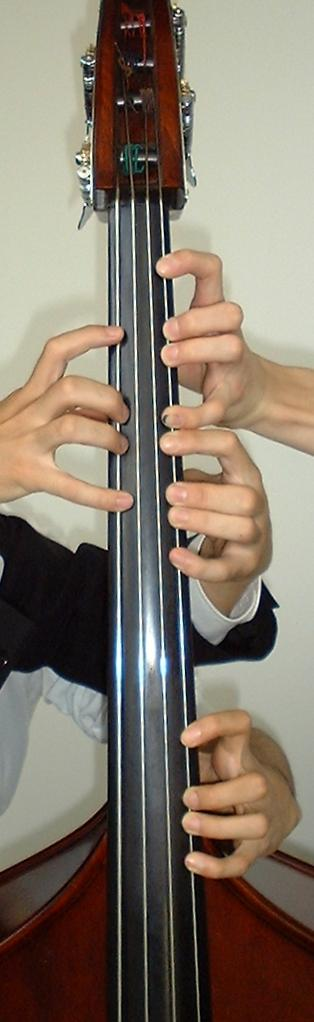
\includegraphics[height=7.5cm]{Pics/Position/4th_3.epsi}\\
{\flushleft\small 図\thefigure : 第IIIポジションは第IIと第IVの間\\}
\end{center}
\end{minipage}
\end{flushleft}

\subsection{音階練習 \label{3rd_scale}}
\begin{music}

\nostartrule
\parindent 0pt
\setclef1{\bass}  
\generalmeter{\meterC}
\generalsignature{2}    
\startpiece
\notes\zchar{19}{ニ長調(D-dur)音階}\enotes
\NOtes\zchar{14}{IV}\ovbkt{!e}{5.5}{3}\zchar{6}{\bf 0}\ql{'D}\zchar{7}{\bf 1}\ql{E}\zchar{8}{\bf 4}\ql{F}\zchar{9}{\bf 0}\ql{G}\enotes
\bar
\NOtes\zchar{10}{\bf 1}\ql{!a}\zchar{11}{\bf 4}\ql{b}\zchar{18}{III}\ovbkt{'c}{3.5}{0}\zchar{12}{\bf 2}\ql{!c}\zchar{13}{\bf 4}\ql{d}\enotes
\bar
\NOtes\zchar{13}{\bf 4}\ql{d}\zchar{12}{\bf 2}\ql{c}\zchar{11}{\bf 4}\zchar{17}{IV}\ovbkt{'b}{5.5}{-3}\ql{!b}\zchar{10}{\bf 1}\ql{a}\enotes
\bar
\NOtes\zchar{9}{\bf 0}\ql{'G}\zchar{8}{\bf 4}\ql{F}\zchar{7}{\bf 1}\ql{E}\zchar{6}{\bf 0}\ql{D}\enotes
\setdoublebar\endpiece
\setclef1{\bass}  
\generalmeter{\meterC}
\generalsignature{3}    
\startpiece
\notes\zchar{19}{イ長調(A-dur)音階}\enotes
\NOtes\zchar{14}{IV}\ovbkt{!f}{5.5}{0}\zchar{9}{\bf 0}\qu{'A}\zchar{9}{\bf 1}\qu{B}\zchar{9}{\bf 4}\qu{C}\zchar{9}{\bf 0}\ql{D}\enotes
\bar
\NOtes\zchar{9}{\bf 1}\ql{'E}\zchar{9}{\bf 4}\ql{F}\zchar{15}{III}\ovbkt{!g}{3.5}{0}\zchar{9}{\bf 2}\ql{'G}\zchar{10}{\bf 4}\ql{!a}\enotes
\bar
\NOtes\zchar{10}{\bf 4}\ql{!a}\zchar{9}{\bf 2}\ql{'G}\zchar{9}{\bf 4}\zchar{14}{IV}\ovbkt{!f}{5.5}{0}\ql{'F}\zchar{9}{\bf 1}\ql{E}\enotes
\bar
\NOtes\zchar{9}{\bf 0}\ql{'D}\zchar{9}{\bf 4}\qu{C}\zchar{9}{\bf 1}\qu{B}\zchar{9}{\bf 0}\qu{A}\enotes
\setdoublebar\endpiece
%\setclef1{\bass}  
%\generalmeter{\meterC}
%\generalsignature{-4}    
%\startpiece
%\notes\zchar{14}{変イ長調(As-dur)音階}\enotes
%\NOtes\zchar{9}{\bf 4}\qu{'A}\zchar{9}{\bf 1}\qu{B}\zchar{9}{\bf 2}\qu{C}\zchar{9}{\bf 4}\ql{D}\enotes
%\bar
%\NOtes\zchar{9}{\bf 1}\ql{'E}\zchar{9}{\bf 2}\ql{F}\zchar{9}{\bf 4}\ql{G}\zchar{10}{\bf 1}\ql{!a}\enotes
%\bar
%\NOtes\zchar{10}{\bf 1}\ql{!a}\zchar{9}{\bf 4}\ql{'G}\zchar{9}{\bf 2}\ql{F}\zchar{9}{\bf 1}\ql{E}\enotes
%\bar
%\NOtes\zchar{9}{\bf 4}\ql{'D}\zchar{9}{\bf 2}\qu{C}\zchar{9}{\bf 1}\qu{B}\zchar{9}{\bf 4}\qu{A}\enotes
%\setdoublebar\endpiece
%\setclef1{\bass}  
%\generalmeter{\meterC}
%\generalsignature{-5}    
%\startpiece
%\notes\zchar{14}{変ニ長調(Des-dur)音階}\enotes
%\NOtes\zchar{9}{\bf 4}\ql{'D}\zchar{9}{\bf 1}\ql{E}\zchar{9}{\bf 2}\ql{F}\zchar{9}{\bf 4}\ql{G}\enotes
%\bar
%\NOtes\zchar{10}{\bf 1}\ql{a}\zchar{11}{\bf 4}\ql{b}\zchar{12}{\bf 1}\ql{c}\zchar{13}{\bf 2}\ql{d}\enotes
%\bar
%\NOtes\zchar{13}{\bf 2}\ql{d}\zchar{12}{\bf 1}\ql{c}\zchar{11}{\bf 4}\ql{b}\zchar{10}{\bf 1}\ql{a}\enotes
%\bar
%\NOtes\zchar{9}{\bf 4}\ql{'G}\zchar{9}{\bf 2}\ql{F}\zchar{9}{\bf 1}\ql{E}\zchar{9}{\bf 4}\ql{D}\enotes
%\setdoublebar\endpiece
\end{music}

%\clearpage

\subsection{フラジオレット(伊: flageoletto)} 
弦長\footnote{弦の端から端までの長さ。通常1メートル強。}の中点は、軽く
触れるだけで開放弦の1オクターヴ上の音が出ます。これをフラジオレットと
呼びます\footnote{ハーモニクス(英: harmonics)とも呼ばれます。}。フラジ
オレットは弦長の\(\frac{1}{3}\)地点、\(\frac{1}{4}\)地点など、弦長
\(\frac{1}{n}\)($n$は2以上の自然数)の地点に存在します。

\clearpage

\begin{flushleft}
\begin{minipage}{140pt}
\subsection{ポジション移動}
\ \ \ \ 「第IV \(\longrightarrow\) 第III」、「第III \(\longrightarrow\) 
第IV」といったように異なるポジション間を移動するときの方法を示します。\\
\ \\
{\bf 上のポジションへ上がるとき}
\begin{enumerate}
\item ポジション移動前(図\addtocounter{figure}{1}\thefigure)
\item 肘を下げる(図\addtocounter{figure}{1}\thefigure)
\item 手首から先を下げる(図\addtocounter{figure}{1}\thefigure)
\end{enumerate}
{\bf 下のポジションへ下がるとき}
\begin{enumerate}
\item ポジション移動前(図\addtocounter{figure}{1}\thefigure)
\item 肘を上げる(図\addtocounter{figure}{1}\thefigure)
\item 手首から先を上げる(図\addtocounter{figure}{1}\thefigure)
\end{enumerate}

\addtocounter{figure}{-6}

\end{minipage}
\hfill
\begin{minipage}{280pt}
\begin{minipage}{80pt}
\addtocounter{figure}{1}
\begin{center}
%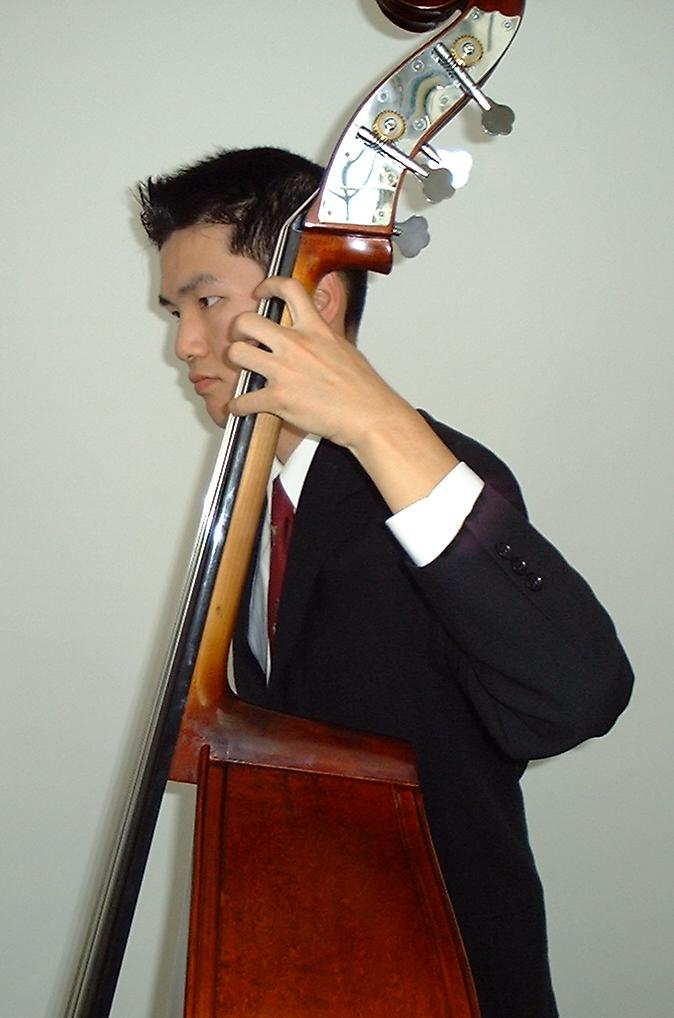
\includegraphics[height=4.5cm]{Pics/Shifting/shiftdown_1.epsi}\\

\includegraphics[width=2cm]{Pics/now_printing.eps}\\
図\thefigure \\
\end{center}
\end{minipage}
\hfill
\begin{minipage}{80pt}
\addtocounter{figure}{1}
\begin{center}
%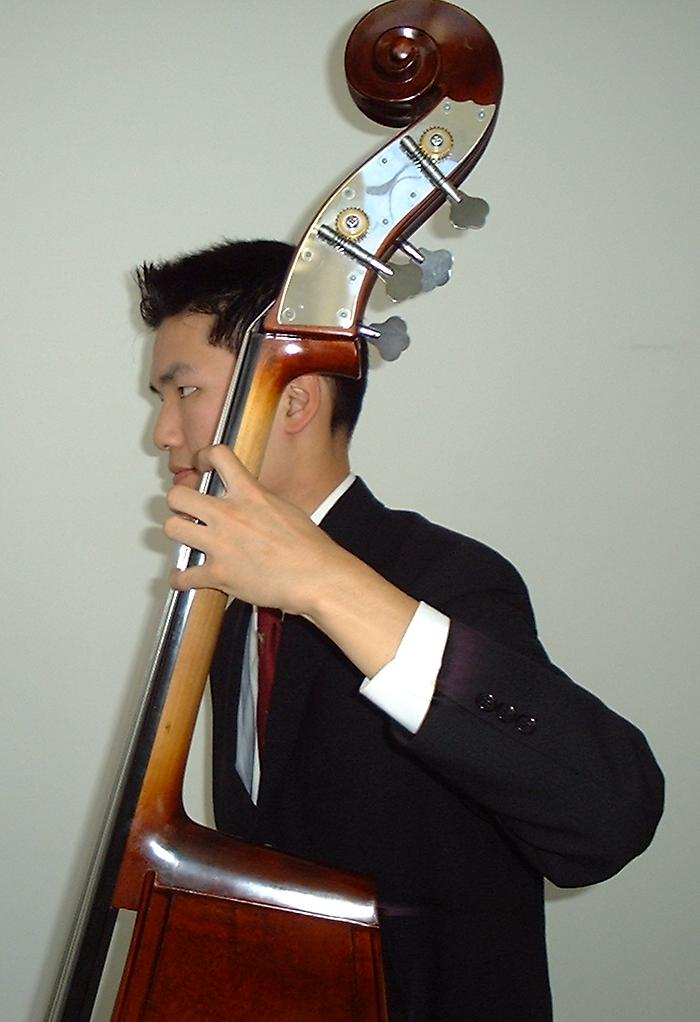
\includegraphics[height=4.5cm]{Pics/Shifting/shiftdown_2.epsi}\\

\includegraphics[width=2cm]{Pics/now_printing.eps}\\
図\thefigure \\
\end{center}
\end{minipage}
\hfill
\begin{minipage}{80pt}
\addtocounter{figure}{1}
\begin{center}
%\includegraphics[height=4.5cm]{Pics/Shifting/shiftdown_3.epsi}\\

\includegraphics[width=2cm]{Pics/now_printing.eps}\\
図\thefigure \\
\end{center}
\end{minipage}

\begin{minipage}{80pt}
\addtocounter{figure}{1}
\begin{center}
%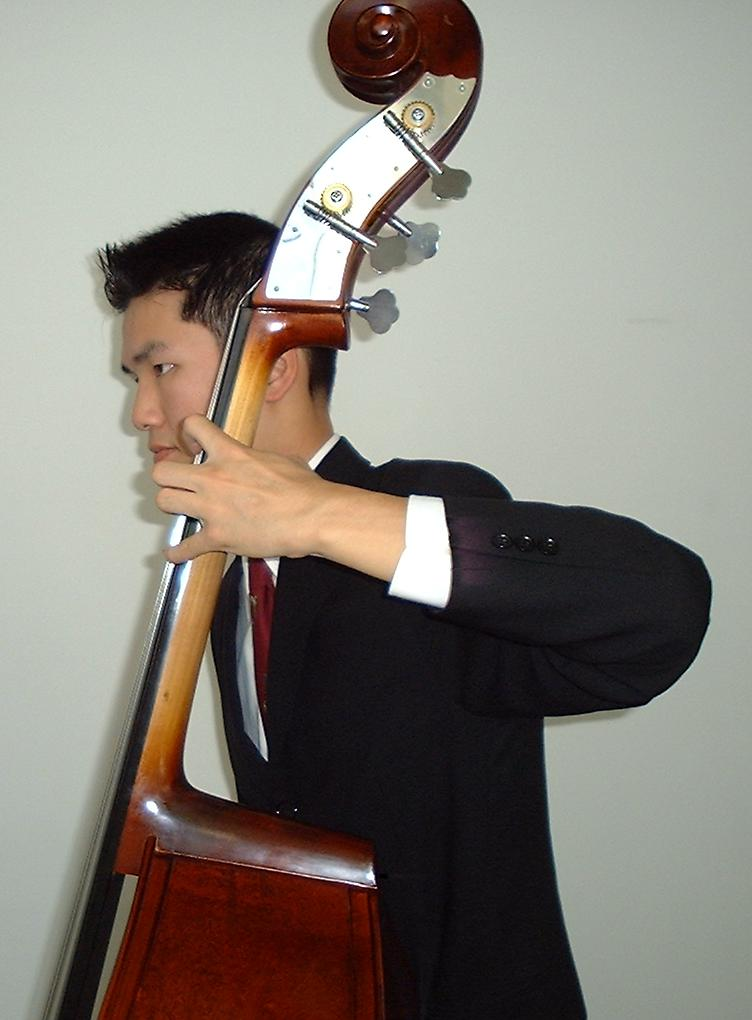
\includegraphics[height=4.5cm]{Pics/Shifting/shiftup_1.epsi}\\

\includegraphics[width=2cm]{Pics/now_printing.eps}\\
図\thefigure \\
\end{center}
\end{minipage}
\hfill
\begin{minipage}{80pt}
\addtocounter{figure}{1}
\begin{center}
%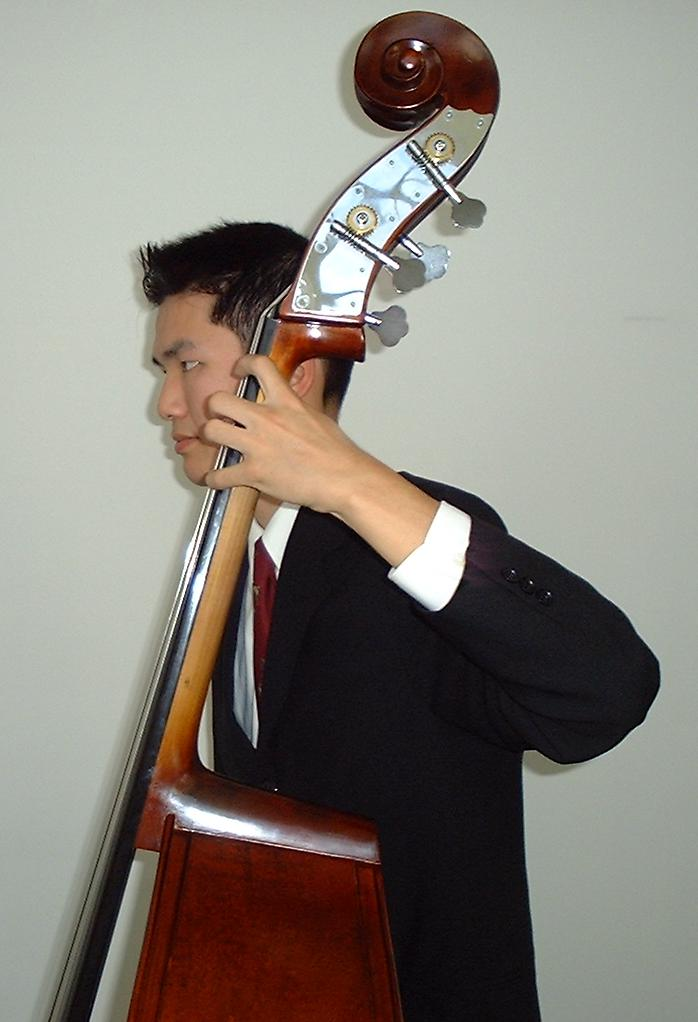
\includegraphics[height=4.5cm]{Pics/Shifting/shiftup_2.epsi}\\

\includegraphics[width=2cm]{Pics/now_printing.eps}\\
図\thefigure \\
\end{center}
\end{minipage}
\hfill
\begin{minipage}{80pt}
\addtocounter{figure}{1}
\begin{center}
%\includegraphics[height=4.5cm]{Pics/Shifting/shiftup_3.epsi}\\

\includegraphics[width=2cm]{Pics/now_printing.eps}\\
図\thefigure \\
\end{center}
\end{minipage}
\end{minipage}
\end{flushleft}

\subsection{調弦(英: tuning)}
第IIIポジションは1の指が弦長の\(\frac{1}{4}\)地点、4の指が
\(\frac{1}{3}\)地点に位置しています。コンサートマスターのAの音に合わせ
て調弦するときには、コントラバスの調弦は第IIIポジションが持つこの性質を
利用して行います。手順は以下の通りです。今日からチューニングメーターな
しでも調弦できるようにしましょう。

\begin{enumerate}
\item 第IVポジションの1の指でD線を軽く押さえます。するとAの音が出る\footnote{弦長\(\frac{1}{3}\)地点なので開放弦の5度上の音が出ます。}ので、この音をコンサートマスターのAに合わせます。
\item 同じ位置を第IIIポジションの4で取り直します。そして、1でA線のフラジオレット音\footnote{弦長\(\frac{1}{4}\)地点なので開放弦の2オクターヴ上の音が出ます。}を出します。この2つの音が同じピッチになるように調整します。
\item 左手を第IIIポジションに置いたままで、A線の4とE線の1が同じピッチのフラジオレット音を出すように調整します。
\item 左手を第IIIポジションに置いたままで、G線の4とD線の1が同じピッチのフラジオレット音を出すように調整します。これで4本の弦すべての調弦が完了します。
\end{enumerate}

演奏会本番では前もってチューニングメーターを用いて調弦をしておきましょう。舞台上で行う調弦は微調整程度で済ませるのが良いステージマナーです。

\subsection{第III・第IVポジションで弾く名曲}
\documentclass{jarticle}
\usepackage{musixdoc}
\startmuflex\makeindex

\begin{document}

\subsubsection*{�⡼�ĥ����: ����ʡ��ǡ֥����͡����饤�͡��ʥϥȥॸ������ K.525 ��Ƭ}
\begin{music}
\nostartrule
\setclef1{\bass}
\generalsignature{1}    
\generalmeter{\meterC}
\parindent 0pt
\startbarno=1
\def\writebarno{\tenrm\the\barno\barnoadd}
\def\raisebarno{2\internote}
\def\shiftbarno{0.1\Interligne}
\systemnumbers
\startpiece\bigaccid
\notes\zchar{16}{\bf Allegro}\enotes
\Notes\ql{'G}\enotes
\notes\ds\cl{'D}\enotes
\Notes\ql{'G}\enotes
\notes\ds\cl{'D}\enotes
\bar
\notes\ibl{0}{'E}{0}\qb{0}{G}\qb{0}{D}\qb{0}{G}\tbl{0}\qb{0}{!b}\enotes
\Notes\ql{d}\qp\enotes
\bar
\Notes\ql{c}\enotes
\notes\ds\cl{a}\enotes
\Notes\ql{c}\enotes
\notes\ds\cl{a}\enotes
\bar
\notes\ibl{0}{c}{-3}\qb{0}{c}\qb{0}{a}\qb{0}{'F}\tbl{0}\qb{0}{!a}\enotes
\Notes\ql{'D}\qp\enotes
\setdoublebar
\endpiece
\end{music}

\endmuflex
\end{document}

\documentclass{jarticle}
\usepackage{musixdoc}
\startmuflex\makeindex

\begin{document}

\subsubsection*{�١��ȡ�������: �������9�� ��ûĴ �ֹ羧�դ��� ��4�ھϤ��}

\begin{music}
\nostartrule
\setclef1{\bass}
\generalsignature{1}    
\generalmeter{\meterfrac32}
\parindent 0pt
\startbarno=595
\def\writebarno{\tenrm\the\barno\barnoadd}
\def\raisebarno{2\internote}
\def\shiftbarno{0.1\Interligne}
\systemnumbers
\startpiece\bigaccid
\Notes\zchar{-5}{\ff}\zchar{18}{\bf Andante maestoso (\metron{\hu}{72})}\hl{'G}\enotes
\bar
\barno=595
\NOtes\wh{'G}\enotes
\Notes\hl{'G}\enotes
\bar
\Notes\hl{'F}\hl{D}\hl{!e}\enotes
\bar
\NOtes\wh{e}\enotes
\Notes\hl{e}\enotes
\bar
\Notes\hl{d}\hl{b}\zchar{-5}{\ppfftwenty sf}\hl{c}\enotes
\alaligne
\NOtes\wh{c}\enotes
\Notes\hl{c}\enotes
\bar
\Notes\hl{b}\enotes
\NOtes\wh{'G}\enotes
\bar
\NOtes\wh{e}\enotes
\Notes\hl{e}\enotes
\bar
\NOTEs\whp{d}\enotes
\setdoublebar
\endpiece
\end{music}

\endmuflex
\end{document}

%\documentclass{jarticle}
\usepackage{musixdoc}
\startmuflex\makeindex

\begin{document}

\subsubsection*{�֥顼�ॹ: �������1�� ��ûĴ ��4�ھϤ��}
\begin{music}
\nostartrule
\setclef1{\bass}
\generalsignature{0}    
\generalmeter{\meterC}
\parindent 0pt
\startbarno=148
\def\writebarno{\tenrm\the\barno\barnoadd}
\def\raisebarno{2\internote}
\def\shiftbarno{0.1\Interligne}
\systemnumbers
\startpiece\bigaccid
\notes\zchar{18}{\bf (Pi\`{u} allegro)}\enotes
\Notes\zchar{-5}{\ff}\hl{eb}\enotes
\bar
\Notes\hl{'EG}\enotes
\bar
\NOtes\zchar{-5}{\ppfftwenty sf}\hlp{a}\enotes
\Notes\qu{'A}\enotes
\bar
\NOtes\zchar{-5}{\ppfftwenty sf}\hlp{a}\enotes
\Notes\ql{'D}\enotes
\alaligne
\Notes\ql{d^deb}\enotes
\bar
\Notes\ql{c'G!a}\qu{'A}\enotes
\bar
\Notes\zchar{-5}{\ppfftwenty sf}\ql{'EG!b}\qu{'B}\enotes
\bar
\Notes\zchar{-5}{\ppfftwenty sf}\ql{'EG!b}\qu{'B}\enotes
\setdoublebar
\endpiece
\end{music}

\endmuflex
\end{document}

\subsubsection*{ヘンデル: オラトリオ「メサイア」より「ハレルヤ」}

\begin{music}
\nostartrule
\setclef1{\bass}
\generalsignature{2}    
\generalmeter{\meterC}
\parindent 0pt
\startbarno=8
\def\writebarno{\tenrm\the\barno\barnoadd}
\def\raisebarno{2\internote}
\def\shiftbarno{0.1\Interligne}
\systemnumbers
\startpiece\bigaccid
\notes\zchar{21}{\bf Allegro}\enotes
\NOtes\zchar{13}{\downbow}\zchar{11}{\bf 4}\zchar{-4}{III}\qlp{a}\enotes
\Notes\zchar{16}{\upbow}\zchar{13}{\bf 2}\cl{c}\ibl{0}{d}{-4}\zchar{16}{\downbow}\zchar{14}{\bf 4}\qb{0}{d}\tbl{0}\zchar{14}{\upbow}\zchar{11}{\bf 4}\qb{0}{a}\qp\enotes
\bar
\NOtes\zchar{13}{\downbow}\zchar{11}{\bf 4}\qlp{a}\enotes
\Notes\zchar{16}{\upbow}\zchar{13}{\bf 2}\cl{c}\ibl{0}{d}{-4}\zchar{16}{\downbow}\zchar{14}{\bf 4}\qb{0}{d}\tbl{0}\zchar{14}{\upbow}\zchar{11}{\bf 4}\qb{0}{a}\ds\ibl{0}{c}{0}\ibbl{0}{c}{0}\zchar{16}{\downbow}\zchar{13}{\bf 2}\qb{0}{c}\tbl{0}\tbbl{0}\zchar{16}{\upbow}\zchar{13}{\bf 2}\qb{0}{c}\enotes
\bar
\Notes\ibl{0}{d}{-4}\zchar{16}{\downbow}\zchar{14}{\bf 4}\qb{0}{d}\tbl{0}\zchar{14}{\upbow}\zchar{11}{\bf 4}\qb{0}{a}\ds\ibl{0}{c}{0}\ibbl{0}{c}{0}\zchar{16}{\downbow}\zchar{13}{\bf 2}\qb{0}{c}\tbl{0}\tbbl{0}\zchar{16}{\upbow}\zchar{13}{\bf 2}\qb{0}{c}\ibl{0}{d}{-4}\zchar{16}{\downbow}\zchar{14}{\bf 4}\qb{0}{d}\tbl{0}\zchar{14}{\upbow}\zchar{11}{\bf 4}\qb{0}{a}\ds\zchar{16}{\upbow}\zchar{13}{\bf 2}\cl{c}\enotes
\bar
\Notes\ibl{0}{d}{-2}\zchar{16}{\downbow}\zchar{14}{\bf 4}\qb{0}{d}\tbl{0}\zchar{16}{\upbow}\zchar{13}{\bf 2}\qb{0}{c}\zchar{-4}{IV}\zchar{14}{\downbow}\zchar{12}{\bf 4}\ql{b}\zchar{14}{\upbow}\zchar{11}{\bf 1}\ql{a}\qp\enotes
\bar
\NOtes\zchar{13}{\downbow}\zchar{11}{\bf 1}\zchar{-4}{\ff}\hl{a}\enotes
\Notes\zchar{15}{\upbow}\zchar{12}{\bf 4}\ql{b}\zchar{16}{\upbow}\zchar{13}{\bf 2}\zchar{-4}{III}\ql{c}\enotes
\bar
\Notes\ibl{0}{'F}{-2}\zchar{16}{\downbow}\zchar{14}{\bf 4}\qb{0}{!d}\tbl{0}\zchar{13}{\upbow}\zchar{10}{\bf 1}\qb{0}{'D}\enotes
\NOtes\zchar{16}{\downbow}\zchar{14}{\bf 4}\hl{d}\enotes
\Notes\zchar{16}{\upbow}\zchar{13}{\bf 2}\ql{c}\zchar{19}{\LARGE \bf A}\enotes
\bar
\NOtes\zchar{14}{\downbow}\zchar{12}{\bf 4}\zchar{-4}{IV}\hl{b}\enotes
\Notes\zchar{14}{\upbow}\zchar{11}{\bf 1}\ql{a}\ds\zchar{-4}{\f}\ibl{0}{c}{0}\ibbl{0}{c}{0}\zchar{16}{\downbow}\zchar{13}{\bf 2}\zchar{-8}{III}\qb{0}{c}\tbl{0}\tbbl{0}\zchar{16}{\upbow}\zchar{13}{\bf 2}\qb{0}{c}\enotes
\bar
\Notes\ibl{0}{d}{-4}\zchar{16}{\downbow}\zchar{14}{\bf 4}\qb{0}{d}\tbl{0}\zchar{14}{\upbow}\zchar{11}{\bf 4}\qb{0}{a}\ds\ibl{0}{c}{0}\ibbl{0}{c}{0}\zchar{16}{\downbow}\zchar{13}{\bf 2}\qb{0}{c}\tbl{0}\tbbl{0}\zchar{16}{\upbow}\zchar{13}{\bf 2}\qb{0}{c}\ibl{0}{d}{-4}\zchar{16}{\downbow}\zchar{14}{\bf 4}\qb{0}{d}\tbl{0}\zchar{14}{\upbow}\zchar{11}{\bf 4}\qb{0}{a}\ds\ibl{0}{c}{0}\ibbl{0}{c}{0}\zchar{16}{\downbow}\zchar{13}{\bf 2}\qb{0}{c}\tbl{0}\tbbl{0}\zchar{16}{\upbow}\zchar{13}{\bf 2}\qb{0}{c}\enotes
\bar
\Notes\ibl{0}{d}{-4}\zchar{16}{\downbow}\zchar{14}{\bf 4}\qb{0}{d}\tbl{0}\zchar{14}{\upbow}\zchar{11}{\bf 4}\qb{0}{a}\ds\ibl{0}{c}{0}\ibbl{0}{c}{0}\zchar{16}{\downbow}\zchar{13}{\bf 2}\qb{0}{c}\tbl{0}\tbbl{0}\zchar{16}{\upbow}\zchar{13}{\bf 2}\qb{0}{c}\ibl{0}{d}{-4}\zchar{16}{\downbow}\zchar{14}{\bf 4}\qb{0}{d}\tbl{0}\zchar{14}{\upbow}\zchar{11}{\bf 4}\qb{0}{a}\enotes
\setdoublebar
\endpiece
\end{music}

